% =============================================================================
% Capítulo 3 — Modelos de Machine Learning para Classificação e Agrupamento
% =============================================================================

 O Capítulo~2 mostrou que as campanhas de ocultação estelar podem produzir diversas curvas de luz, sendo número suficiente para que haja dificuldade na análise completa e minuciosa. Cada curva pode ser resumida por um conjunto de características como profundidade da queda, estatísticas de ruído, entre outros. A questão é: \emph{a partir dessa descrição numérica de uma curva, é possível decidir automaticamente se ela contém ou não uma ocultação?} Trata-se de um problema de \textbf{classificação binária}, e os métodos de \textit{Machine Learning} são as ferramentas naturais para resolvê-lo. \ia{Com isso, os objetivos deste capítulo são: definir e situar os modelos de Machine Learning como ferramentas de descobertas e classificações no contexto científico; formalizar o problema de classificação (espaço de atributos, rótulos, regiões de decisão); apresentar os principais modelos utilizados na \textit{pipeline}; e, por fim, discutir algoritmos de otimização, engenharia de características, validação de modelos e os riscos de falsos resultados.}

% -----------------------------------------------------------------------------
\section{Conceitos fundamentais de Machine Learning}
\label{sec:fundamentos_ml}

\subsection{Definição e papel do aprendizado de máquina}

O \textit{Machine Learning} (ML), ou aprendizado de máquina, é uma área na qual os sistemas "aprendem" a partir de dados, sem serem explicitamente programados para cada tarefa \citep{geron2019maos}. Em vez de regras fixas codificadas à mão, um algoritmo de ML é alimentado com informações e \textbf{ajusta seus próprios parâmetros} (por exemplo, coeficientes de uma combinação linear) para capturar padrões ou relações nos dados. Esse processo de ajuste é o que se chama de \textbf{treinamento}; ao final, o modelo está "treinado" e pode ser aplicado a novas informações. O objetivo é permitir que o sistema melhore seu desempenho à medida que mais dados ou mais iterações estejam disponíveis, especialmente em problemas sem solução analítica fechada ou com grandes volumes de dados.

No contexto científico, o ML costuma ser visto como "caixa-preta" que produz previsões sem explicação. Essa visão reflete usos industriais em que a precisão preditiva prevalece sobre a interpretabilidade. Em ciência, porém, o ML pode ir além: atuando como ferramenta de descoberta, revelando padrões que podem ser incorporados a uma teoria formal de causa e efeito. O papel do ML não é substituir a teoria, mas auxiliar na sua formulação, identificando os padrões que a teoria buscará explicar. Segundo \cite{lopez2020ml}, por exemplo, o uso do ML na ciência pode ser agrupado em algumas funções típicas:

\textbf{Sugerir a existência de algo novo:} ML pode encontrar padrões não previstos, indicando a existência de relações ainda não descobertas. Em matemática, algoritmos já auxiliaram a conjecturar teoremas que depois foram demonstrados formalmente \citep{gryak2018conjugacy}.

\textbf{Descobrir o grau de importância das variáveis:} técnicas como \textit{Mean Decrease Accuracy} (MDA) permitem avaliar o impacto de cada variável (\textbf{feature}, ou característica numérica de entrada) na predição. A ideia é treinar o modelo, medir o desempenho (por exemplo, via acurácia), embaralhar uma variável por vez e verificar se o desempenho cai; se cair, a variável é importante \citep{liu2004comparative}. Assim, o ML identifica quais variáveis devem compor explicações teóricas, mesmo sem revelar o mecanismo causal.

\textbf{Explorar relações de causa e efeito:} um modelo pode ser ajustado com dados nos quais um determinado efeito está ausente. Depois, quando esse efeito passa a atuar, o modelo continua produzindo previsões baseadas no cenário anterior. Se as observações reais passarem a divergir das previsões, essa diferença pode ser um indício de que o efeito alterou o sistema, sugerindo possíveis relações causais.

\textbf{Redução e simplificação:} em dados multidimensionais, técnicas de redução de dimensionalidade — por exemplo, a Análise de Componentes Principais (PCA) — projetam os dados em um espaço de menor dimensão, tornando mais evidentes padrões, agrupamentos e relações entre observações, o que favorece a interpretação dos resultados.

\textbf{Encontrar padrões desconhecidos:} o ML pode atuar na detecção de eventos raros ou anomalias em grandes volumes de dados - por exemplo, na triagem automática de ocultações estelares em levantamentos astronômicos - indicando onde vale a pena investigar, mesmo sem explicar o mecanismo.

Neste trabalho, o ML atua sobretudo na função de \textbf{encontrar padrões desconhecidos} e de \textbf{descobrir o grau de importância das variáveis} (importância das \textit{features} nos ensembles de árvores), em apoio à decisão do pesquisador sobre quais curvas merecem análise detalhada.

\subsection{Aprendizado supervisionado versus não supervisionado}

A taxonomia usual divide o ML em dois cenários, conforme a natureza dos dados:

\begin{itemize}
	\item \textbf{Supervisionado:} cada exemplo possui um rótulo (classe ou valor numérico). Tarefas típicas: classificação (rótulo discreto) e regressão (rótulo contínuo). Exemplos: filtro de spam, previsão de preços.
	\item \textbf{Não supervisionado:} os dados não possuem rótulos. Tarefas típicas: agrupamento (clustering), detecção de anomalias, redução de dimensionalidade. Exemplos: segmentação de clientes, identificação de \textit{outliers} (anomalias).
\end{itemize}

Neste trabalho, o foco é o \textbf{paradigma supervisionado}, em particular a \textbf{classificação binária}. No aprendizado supervisionado, o objetivo é encontrar uma função \(f\) que mapeie cada entrada \(\vec{x}\) (por exemplo, o vetor de características de uma curva de luz) a um rótulo \(y\) (por exemplo, "ocultação presente" ou "ausente"). Os rótulos usados no treinamento vêm da classificação já conhecida dos dados (a chamada \textbf{verdade de campo}, ou \textit{ground truth} - por exemplo, a análise prévia de um especialista ou o catálogo). O objetivo é que \(f\) \textbf{generalize} bem, ou seja, que erre pouco em dados novos que não foram usados no ajuste. A detecção de ocultações estelares é formulada exatamente assim: a curva de luz contém um evento de ocultação (classe positiva, \(y=1\)) ou não (classe negativa, \(y=0\)). Os classificadores (Regressão Logística, Random Forest, XGBoost, CatBoost) recebem vetores de características extraídos das curvas e produzem uma classe ou uma probabilidade de classe, permitindo triagem e priorização automáticas no fluxo da \textit{pipeline} \ia{(Capítulo 4)}.

% -----------------------------------------------------------------------------
\section{O problema da classificação supervisionada}
\label{sec:problema_classificacao}
\label{sec:reglin_didatica}

Em notação matemática, uma amostra rotulada é representada pela tupla \(Z = (X, Y)\). Aqui \(X = \{\vec{x}_1, \vec{x}_2, \ldots, \vec{x}_n\}\) é o conjunto de \textbf{vetores de características}: cada \(\vec{x}_i \in \mathbb{R}^d\) é um vetor com \(d\) números que resumem, no caso deste trabalho, uma curva de luz (amplitude, mínimo do fluxo suavizado, distância entre centróides, etc.). O número \(d\) é a "dimensionalidade'' do problema (neste caso, 14 ou 28 features). O conjunto \(Y = \{y_1, y_2, \ldots, y_n\}\) contém os \textbf{rótulos}: a classificação verdadeira de cada exemplo, com \(y_i \in \{0,1\}\) no caso binário (0 = sem ocultação, 1 = com ocultação).

Um \textbf{classificador} é uma função \(f \colon \mathbb{R}^d \longrightarrow \{0,1\}\) (ou, em geral, \(\{1,\ldots,c\}\) para \(c\) classes) que, dado um vetor \(\vec{x}\), prediz um rótulo \(y\). Em muitos modelos, \(f\) produz primeiro uma \textbf{probabilidade} de a classe ser positiva; a decisão final é então "positivo"~se essa probabilidade for maior ou igual a 50 \%, e "negativo"~caso contrário. O uso do valor 0,5 é intuitivo, mas cabe frisar que é arbitrário e dependerá do objetivo do modelo que está sendo treinado (esse limite decisório é chamado de 'threshold' nas pipelines de ML, ou $\tau$, e será melhor explorado mais adiante). 

A função \(f\) divide o espaço \(\mathbb{R}^d\) em \textbf{regiões de decisão}: \(R_k = \{\vec{x} \in \mathbb{R}^d \mid f(\vec{x}) = k\}\). Cada região corresponde a uma classe. O objetivo do treinamento é estimar \(f\) a partir dos dados \((X,Y)\) de modo que \(f\) generalize bem para novos exemplos não vistos.

Antes de apresentar os modelos de classificação, convém fixar a ideia de treinamento como minimização de uma função de custo. O exemplo mais natural de ser explorado é a \textbf{regressão linear}. O modelo $y_i = \beta_0 + \beta_1 x_i + \epsilon_i$ descreve o comportamento médio de uma variável resposta $y$ dado $x$, com erro $\epsilon_i$ (Figura~\ref{fig:linear}).

\begin{figure}[htbp]
\begin{center}
	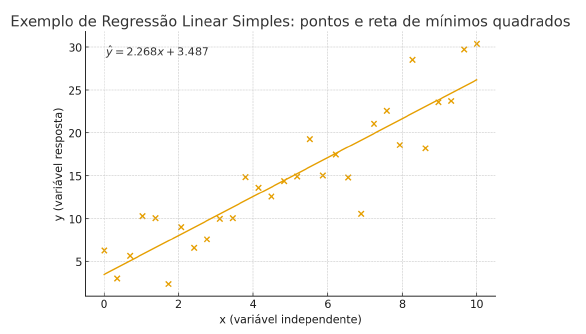
\includegraphics[scale=0.9]{pngs/exemplo_regressaoLinear.png}
\caption{Exemplo ilustrativo de regressão linear simples (dados genéricos, não referentes a curvas de luz de ocultação) \citep{Levada2026}.}
\label{fig:linear}
\end{center}
\end{figure}

Os parâmetros são estimados pelo método dos \textbf{mínimos quadrados}, que constitui o primeiro exemplo de algoritmo de otimização nesta dissertação. No caso mais simples ($\mathbb{R}^2$), o modelo é $y = \alpha + \beta x$ e a função de custo é
\[
J(\alpha,\beta) = \sum_{i=1}^{n} (y_i - \alpha - \beta x_i)^2,
\]
minimizada pela condição $\partial J / \partial \alpha = 0$, $\partial J / \partial \beta = 0$. A generalização para múltiplas variáveis ($d$ dimensões) segue naturalmente em notação vetorial. O modelo prediz $\hat{\vec{y}} = X\vec{\theta}$, com $X$ a matriz de dados (cada linha é um exemplo, cada coluna uma variável) e $\vec{\theta}$ o vetor de parâmetros. A função de custo torna-se
\[
J(\vec{\theta}) = (\vec{y} - X\vec{\theta})^\top (\vec{y} - X\vec{\theta}) = \sum_{i=1}^{n} \big( y_i - \vec{\theta}^\top \vec{x}_i \big)^2.
\]
A condição de mínimo, $\nabla_{\vec{\theta}} J = \vec{0}$, fornece a \textbf{equação normal}:
\[
X^\top (X\vec{\theta} - \vec{y}) = \vec{0} \quad \Longrightarrow \quad \vec{\theta}^* = (X^\top X)^{-1} X^\top \vec{y}.
\]
Após estimar $\vec{\theta}^*$, o modelo pode predizer $\vec{y}$ para novos dados de entrada \citep{geron2019maos, Levada2026}.

Apesar dos problemas de regressão servirem de excelente passo inicial para se compreender as métricas e interpretações básicas dos modelos de ML, para problemas de classificação, não usamos regressão linear diretamente - a solução completa desses problemas podem ser acompanhadas no capítulo 2 de \citep{Levada2026}. A \textbf{Regressão Logística} mantém a combinação linear, mas mapeia a saída ao intervalo $(0,1)$ por uma função sigmoide e utiliza o custo de entropia cruzada, para o qual \ia{\textbf{não existe solução fechada}} (o treinamento é feito por algoritmos iterativos - Seção~\ref{sec:otimizacao}).

% -----------------------------------------------------------------------------
\section{Modelos de classificação utilizados na pipeline}
\label{sec:modelos_classificacao}

\subsection{Regressão Logística}

A Regressão Logística é um classificador probabilístico. Similarmente à Regressão Linear, este modelo calcula uma soma ponderada das características de entrada, mas, em vez de gerar o resultado diretamente, gera a \textit{logística} (função sigmoide) desse resultado \citep{geron2019maos}. Em outras palavras, ele transforma combinações lineares de características em probabilidades válidas.

Suponha um problema de classificação no qual se deseja identificar uma ocultação em uma curva de luz a partir de uma única informação: o \textbf{tamanho da queda máxima do fluxo}. Curvas com maiores quedas possuem maior probabilidade de conter a ocultação. A figura a seguir ilustra a aplicação da regressão linear em dados bem comportados.

\begin{figure}[htbp]
    \centering
    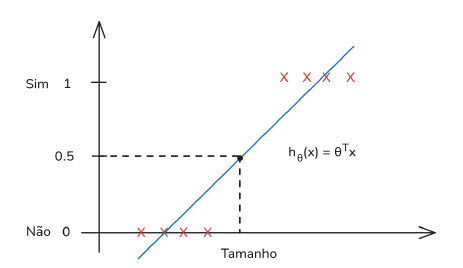
\includegraphics[width=0.5\linewidth]{pngs/regressao_linear_ex1.png}
\caption{Aplicação da regressão linear ao problema de classificação binária: a reta produz saídas fora do intervalo $[0,1]$ \citep{Levada2026}. Nosso conjunto de dados mostra quatro amostras de curvas de luz com grandes amplitudes e outras quatro com baixas amplitudes. Nesse exemplo simples, o valor de 0,5 para o recorte da reta divide perfeitamente as duas classificações.}
    \label{fig:reglin_classif_ex1}
\end{figure}

Nesse caso, teríamos infinitos valores sob uma reta para a variável de saída. \ia{Notadamente,} a solução mais intuitiva seria considerar um limiar simples na metade da reta. No entanto, suponha que, no mesmo conjunto de dados, tivéssemos um elemento \textit{outlier}, uma anomalia. A Figura~\ref{fig:reglin_classif_ex2} ilustra a situação: o limiar que antes funcionava deixa de ser útil, pois agora a metade da reta passa a considerar um ponto positivo como negativo ao mesmo tempo que varios pontos positivos ficam proximos do limiar de decisão (e apenas o outlier se encontra confortavelmente longe das curvas consideradas negativas), gerando dúvida para o analista que estuda os dados.

\begin{figure}[htbp]
    \centering
    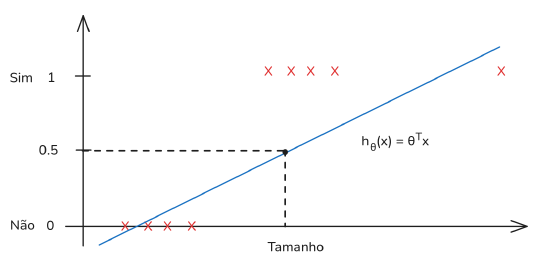
\includegraphics[width=0.5\linewidth]{pngs/regressao_linear_ex2.png}
    \caption{O mesmo problema anterior, mas com a adição de um \textit{outlier}. Uma das curvas possui tamanho de amplitude muito diferente da escala normal, possivelmente resultado da falta de normalização. Veja como a reta de regressão se desloca e o limiar 0,5 passa a classificar incorretamente \citep{Levada2026}.}
    \label{fig:reglin_classif_ex2}
\end{figure}

O que podemos ver é a reta de regressão pode sofrer alterações significativas com a inclusão de novos pontos, evidenciando sua sensibilidade aos dados observados. \ia{Além disso,} a regressão linear pode gerar valores fora do intervalo [0,1], incompatíveis com a interpretação probabilística. \ia{Dessa forma,} sua sensibilidade a outliers e a ausência de uma saída naturalmente probabilística fazem da regressão linear uma abordagem inadequada para tarefas de classificação.

\ia{Nesse sentido,} a regressão logística funcionará de forma similar a modelos lineares (saída contínua), mas será adaptado. O primeiro ponto será a interpretação probabilística: a combinação linear \(\vec{\theta}^\top \vec{x}\) será mapeada pela logística ao intervalo \((0,1)\), permitindo a interpretação como a probabilidade da classe ser positiva \citep{Levada2026}. 

Em notação vetorial, seja \(\vec{\theta}\) o vetor de parâmetros  e \(\vec{x}\) o vetor de atributos; a probabilidade predita é
\[
\hat{p} = h_{\vec{\theta}}(\vec{x}) = \sigma(\vec{\theta}^\top \vec{x}) = \frac{1}{1 + e^{-\vec{\theta}^\top \vec{x}}}.
\]
A decisão é: classe 1 se \(\hat{p} \geq 0{,}5\), caso contrário classe 0. Isso pois a saída continuará continua, mas dessa vez limitada entre 0 e 1. \ia{Vale lembrar, também,} que o valor de 0,5 pode ser alterado a depender da calibração do modelo\ia{, como discutido no início do capítulo}. 

O segundo ponto a ser adaptado será quanto ao treinamento. \ia{Nesse sentido,} passa-se a utilizar outra função de custo ao invés dos mínimo quadrados: a \textbf{entropia cruzada} (ou \textit{log loss}). Essa medida penaliza predições distantes do rótulo real. Por exemplo, se temos uma curva positiva (ocultação presente), e o modelo prediz uma probabilidade baixa de haver ocultação, o custo deverá ser alto. 

\[
loss = - [y \log{p} + (1-y) \log{(1-p)}]
\] onde p é a probabilidade prevista pelo modelo e a perda (loss) deverá ser aplicada a um único ponto. Ou seja, para um conjunto de \(m\) exemplos, com rótulos \(y^{(i)} \in \{0,1\}\) e probabilidades preditas \(\hat{p}^{(i)}\), a função é
\begin{equation}
J(\vec{\theta}) = -\frac{1}{m} \sum_{i=1}^{m} \left[ y^{(i)} \log(\hat{p}^{(i)}) + (1 - y^{(i)}) \log(1 - \hat{p}^{(i)}) \right].
\end{equation}


A minimização de \(J(\vec{\theta})\) é equivalente à maximização da log-verossimilhança (MLE), de modo que os parâmetros estimados são estatisticamente ótimos sob o modelo probabilístico assumido \citep{geron2019maos, Levada2026}. O ajuste é realizado por gradiente descendente (veremos mais detalhes sobre os algoritmos de otimização na Seção~\ref{sec:otimizacao}). O gradiente de \(J\) em relação a \(\vec{\theta}\) pode ser escrito na forma vetorial
\[
\nabla_{\vec{\theta}} J(\vec{\theta}) = \frac{1}{m} X^\top \big( \sigma(X\vec{\theta}) - \vec{y} \big),
\]
onde \(X\) é a matriz de dados e \(\vec{y}\) o vetor de rótulos. A atualização dos parâmetros em cada iteração segue a \textbf{direção oposta ao gradiente} (direção de maior descida do custo), com passo controlado pela \textbf{taxa de aprendizado} \(\eta\) (análogo ao passo de um método numérico de minimização). \ia{Trata-se, portanto, de uma medida sobre o quão distante da realidade estão as previsões do modelo.}

\vspace{0.3cm}
\noindent\textbf{Exemplo numérico: uma iteração do gradiente descendente.}
Para tornar o mecanismo concreto, considere $m = 4$ curvas com uma única feature $x$ (amplitude da queda de fluxo, normalizada entre 0 e 1) e rótulos $y$ (0 = sem ocultação, 1 = com ocultação):

\begin{table}[htbp]
\centering
\small
\begin{tabular}{cccc}
\hline
Curva & $x$ & $y$ & $\hat{p}$ (inicial) \\
\hline
1 & 0{,}2 & 0 & 0{,}50 \\
2 & 0{,}4 & 0 & 0{,}50 \\
3 & 0{,}7 & 1 & 0{,}50 \\
4 & 0{,}9 & 1 & 0{,}50 \\
\hline
\end{tabular}
\caption{Dados do exemplo numérico da Regressão Logística (valores ilustrativos).}
\label{tab:exemplo_logistica}
\end{table}

Inicializamos $\theta_0 = 0$ e $\theta_1 = 0$. Como $\sigma(0) = 0{,}5$, todas as curvas recebem probabilidade $\hat{p} = 0{,}5$ e o custo inicial é $J = -\log(0{,}5) \approx 0{,}693$. Os gradientes são $\partial J / \partial \theta_0 = \frac{1}{4}\sum_i (\hat{p}_i - y_i) = 0$ e $\partial J / \partial \theta_1 = \frac{1}{4}\sum_i (\hat{p}_i - y_i)\,x_i = -0{,}15$. Com taxa de aprendizado $\eta = 1{,}0$, a atualização dá $\theta_1 \leftarrow 0 - 1{,}0 \times (-0{,}15) = 0{,}15$. Recalculando as probabilidades com o novo $\theta_1$, obtemos $\hat{p}_1 = \sigma(0{,}03) \approx 0{,}507$, $\hat{p}_2 \approx 0{,}515$, $\hat{p}_3 \approx 0{,}526$ e $\hat{p}_4 \approx 0{,}534$. O custo cai para $J \approx 0{,}685$. Uma única iteração já empurrou as probabilidades na direção correta: as curvas com maior amplitude (3 e 4, positivas) receberam $\hat{p}$ ligeiramente maior que as negativas. Após centenas de iterações, a separação se consolida.
\vspace{0.3cm}

Sem nenhuma restrição, a Regressão Logística é livre para atribuir pesos enormes a qualquer feature --- inclusive ao ruído. Se uma curva de treino por acaso tem um pico espúrio que coincide com a classe positiva, o modelo pode atribuir peso grande a essa flutuação; na hora de classificar curvas novas, esse peso exagerado prejudica a predição. Esse é o problema do \textbf{sobreajuste} (overfitting, discutido em detalhe na Seção~\ref{sec:overfitting}): o modelo ``decorou'' particularidades do treino em vez de aprender o padrão geral.

A solução é a \textbf{regularização}: impor um custo adicional aos pesos grandes, forçando o modelo a manter coeficientes moderados e a distribuir a ``explicação'' entre múltiplas \textit{features} em vez de apostar tudo em uma \citep{geron2019maos, Levada2026}. As três formas principais são:

\begin{itemize}
	\item \textbf{Ridge (\(\ell_2\)):} adiciona ao custo o termo \(\frac{\alpha}{2} \sum_j \theta_j^2\). Os coeficientes são \textit{encolhidos} em direção a zero, mas raramente se anulam - todos os atributos permanecem no modelo. Funciona bem com \textit{features} correlacionadas, reduzindo o sobreajuste sem descartar características.

	\item \textbf{Lasso (\(\ell_1\)):} adiciona \(\alpha \sum_j |\theta_j|\). Tende a \textbf{zerar} coeficientes de atributos irrelevantes, atuando como seleção automática de variáveis. Em contrapartida, pode comportar-se de forma errática com muitas variáveis correlacionadas (tendendo a escolher apenas uma) ou quando o número de variáveis supera o de instâncias. A função de custo não é diferenciável em \(\theta_j = 0\) (algoritmos de otimização não sabem a direção do próximo passo), exigindo subgradientes na otimização.

	\item \textbf{Elastic Net:} combina as penalidades Ridge e Lasso com uma taxa de mistura, unindo os benefícios de ambas. É recomendado quando há muitas variáveis correlacionadas.
\end{itemize}

Existe uma interpretação elegante dessas penalidades do ponto de vista bayesiano (Estimativa MAP --- \textit{Maximum A Posteriori}). Regularizar equivale a assumir uma crença prévia (\textit{prior}) sobre os valores dos coeficientes do modelo \emph{antes} de ver os dados. No Ridge, essa crença é uma \textbf{distribuição Gaussiana} centrada em zero: acredita-se que os pesos são provavelmente pequenos, mas não necessariamente nulos --- as caudas suaves da Gaussiana permitem valores moderados (Figura~\ref{fig:gaussLaplace}). No Lasso, a crença é uma \textbf{distribuição de Laplace}, que tem um pico afiado em zero: acredita-se que muitos pesos \emph{são} zero, e apenas alguns poucos são relevantes --- daí o efeito de seleção automática de variáveis \citep{geron2019maos, Levada2026}.

O hiperparâmetro \(\alpha\) (ou \(C = 1/\alpha\)) controla a força da penalização: \(\alpha\) grande significa uma crença prévia forte de que os pesos devem ser pequenos; \(\alpha\) pequeno deixa o modelo mais livre. A escolha de \(\alpha\) é feita por \textbf{validação cruzada}: treina-se o modelo com diferentes valores de \(\alpha\) e seleciona-se aquele de melhor desempenho médio nas partições de validação (as \emph{dobras}, ou \textit{folds}, definidas na Seção~\ref{sec:validacao_modelos}) \citep{geron2019maos}.

É essencial \textbf{escalonar} as \textit{features} (e.g.\ StandardScaler) antes de aplicar Ridge ou Lasso, pois ambas as penalidades são sensíveis à escala dos dados: um atributo medido em quilômetros terá coeficiente numericamente muito diferente do mesmo atributo medido em metros, e a penalização tratará ambos de forma desigual. Nesta dissertação, utiliza-se Ridge ou Lasso na Regressão Logística, conforme documentado no Apêndice~\ref{ap:hiperparametros}.

\begin{figure}[!h]
    \centering
    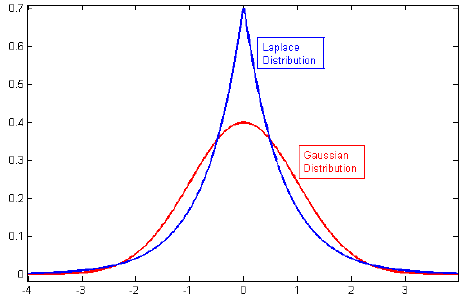
\includegraphics[width=0.5\linewidth]{Tese/pngs/Comparison-of-Gaussian-and-Laplace-distributions.png}
    \caption{Comparação entre as distribuições Gaussiana e de Laplace, que correspondem aos priors assumidos sobre os parâmetros na interpretação bayesiana das regularizações Ridge e Lasso, respectivamente.}
    \label{fig:gaussLaplace}
\end{figure}


A Regressão Logística serve de base conceitual para entender classificadores probabilísticos e foi também treinada e avaliada na \textit{pipeline} desta dissertação, junto com os demais modelos (Random Forest, XGBoost, CatBoost), que tipicamente oferecem melhor desempenho em dados tabulares e fornecem importância de variáveis. A função sigmoide \(\sigma(z) = 1/(1+e^{-z})\) está ilustrada na Figura~\ref{fig:sigmoide}.

\begin{figure}[htbp]
\begin{center}
	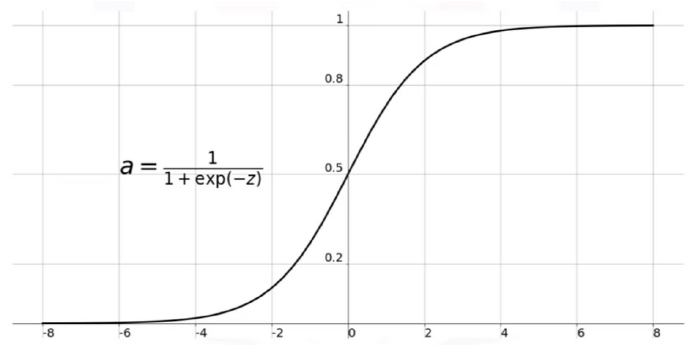
\includegraphics[scale=0.85]{pngs/sigmoide.png}
\caption{Função sigmoide \(\sigma(z) = 1/(1+e^{-z})\).}
\label{fig:sigmoide}
\end{center}
\end{figure}

\subsection{Árvores de decisão e critérios de impureza}

Os modelos Random Forest, XGBoost e CatBoost são baseados em \textbf{árvores de decisão}. Uma árvore de decisão é um classificador que funciona como um fluxograma: em cada "nó"~ pergunta-se o valor de uma das características (por exemplo, "o mínimo do fluxo suavizado é menor que 0,85?"); conforme a resposta, segue-se por um dos dois ramos até um novo nó ou até uma "folha", que devolve a classe predita. O espaço de entradas (vetores de características) fica assim particionado em regiões (hiper-retângulos), cada uma associada a uma classe \citep{Levada2026}. Uma das maiores vantagens é a \textbf{interpretabilidade}: as regras podem ser lidas e aplicadas manualmente, em contraste com modelos opacos como redes neurais. O \textit{scikit-learn} \citep{ScikitLearn2011} utiliza o algoritmo \textbf{CART} (\textit{Classification and Regression Trees}), que produz árvores binárias e escolhe, em cada nó, a divisão que maximiza a pureza dos nós filhos \citep{geron2019maos}. Os dois critérios de impureza mais usados para classificação são o \textbf{coeficiente de Gini} e a \textbf{entropia}. Para um nó \(i\) com proporções \(p_{i,k}\) de exemplos na classe \(k\) (com \(k=1,\ldots,c\) classes):
\begin{equation}
G_i = 1 - \sum_{k=1}^{c} p_{i,k}^2, \qquad
H_i = -\sum_{k=1}^{c} p_{i,k} \log_2(p_{i,k}) \quad (\text{convenção } 0\log 0 = 0).
\end{equation}
Nessas expressões, \(G_i\) é o coeficiente de Gini e \(H_i\) é a \textbf{entropia} do nó \(i\): ambos medem a impureza, ou seja, o quanto as classes estão misturadas naquele nó. Os dois valem zero quando o nó é puro (todos os exemplos pertencem a uma única classe) e crescem à medida que as classes ficam mais equilibradas entre si.

O Gini tende a isolar a classe mais frequente; a entropia tende a produzir árvores mais equilibradas. A divisão é feita de modo a maximizar a redução da impureza (ganho de informação). Árvores de decisão são instáveis e sensíveis a pequenas variações nos dados; sem restrições, tendem ao sobreajuste. Para regularizar, utilizam-se critérios de parada como profundidade máxima (\textit{max\_depth}) e número mínimo de amostras por nó ou por folha (\textit{min\_samples\_leaf}) \citep{geron2019maos}. A \textbf{poda} (\textit{pruning}) pode ser aplicada após o crescimento completo, removendo ramos que não contribuem significativamente para a capacidade preditiva \citep{Levada2026}.

\vspace{0.3cm}
\noindent\textbf{Exemplo numérico: redução de impureza de Gini em uma divisão.}
Considere um nó contendo $8$ curvas de luz de treino, sendo $4$ positivas (com ocultação) e $4$ negativas. Como as classes estão perfeitamente misturadas, a impureza é máxima para o caso binário:
\[
G_{\text{nó}} = 1 - \left[\left(\tfrac{4}{8}\right)^2 + \left(\tfrac{4}{8}\right)^2\right] = 1 - 0{,}5 = 0{,}5.
\]
A árvore testa então uma divisão candidata --- por exemplo, ``profundidade da queda $> 0{,}5$?'' --- que separa as $8$ curvas em dois nós-filhos:
\begin{itemize}
	\item \textbf{Filho da esquerda} ($3$ curvas, todas positivas): $G_{\text{esq}} = 1 - \left[1^2 + 0^2\right] = 0$ (nó \emph{puro}).
	\item \textbf{Filho da direita} ($5$ curvas, $1$ positiva e $4$ negativas): $G_{\text{dir}} = 1 - \left[\left(\tfrac{1}{5}\right)^2 + \left(\tfrac{4}{5}\right)^2\right] = 1 - 0{,}68 = 0{,}32$.
\end{itemize}
A impureza após a divisão é a média \textbf{ponderada} pelo número de exemplos em cada filho:
\[
G_{\text{div}} = \frac{3}{8}\times 0 + \frac{5}{8}\times 0{,}32 = 0{,}20,
\]
e o \textbf{ganho} (redução de impureza) é $\Delta G = G_{\text{nó}} - G_{\text{div}} = 0{,}50 - 0{,}20 = 0{,}30$. A divisão deixou os nós mais ``puros'' (o da esquerda já decide com certeza pela classe positiva). O algoritmo CART avalia todos os cortes candidatos de todas as \textit{features} e escolhe aquele que produz o \emph{maior} ganho; o processo se repete em cada nó-filho até atingir um critério de parada.
\vspace{0.3cm}

\subsection{Random Forest (Floresta Aleatória)}

Random Forest é um método de \textbf{ensemble}: em vez de uma única árvore, treina-se um grande número de árvores de decisão (por exemplo, centenas), cada uma em uma \textbf{amostra aleatória} dos dados (amostragem com reposição, ou \textit{bootstrap}) e usando, em cada divisão de nó, apenas um subconjunto aleatório das características \citep{geron2019maos, Levada2026}. A predição final é obtida por \textbf{votação majoritária}: cada árvore "vota" em uma classe e escolhe-se a classe que recebeu mais votos. A força da floresta está na \textbf{descorrelação} entre as árvores. Aqui, \textbf{\textit{bagging}} (de \textit{bootstrap aggregating}) é a técnica de treinar cada árvore em uma amostra distinta dos dados, sorteada com reposição, e depois agregar as predições por votação: como cada árvore vê um conjunto ligeiramente diferente, elas erram em casos diferentes. O \textit{bagging} e a escolha aleatória de atributos em cada nó garantem essa diversidade; ao agregar centenas de árvores, o modelo mantém o baixo viés das árvores individuais e reduz drasticamente a \textbf{variância}. Uma vantagem colateral é a estimativa \textbf{out-of-bag} (OOB): como cada árvore é treinada em aproximadamente 63\% dos dados (amostragem com reposição), cerca de 37\% das instâncias ficam "fora da bolsa"~para cada árvore e podem ser usadas como conjunto de validação interno, permitindo estimar o erro de generalização sem um conjunto de teste separado \citep{geron2019maos}. Uma variante ainda mais aleatória são as \textbf{Extra-Trees} (\textit{Extremely Randomized Trees}): em vez de procurar o melhor ponto de corte em cada atributo, sorteiam limiares ao acaso e ficam com o melhor entre os sorteados. Isso acelera o treinamento e pode reduzir ainda mais a variância, ao custo de um viés ligeiramente maior \citep{geron2019maos}.

A aleatoriedade em dois níveis --- nos dados e nos atributos --- reduz a correlação entre as árvores e diminui a \textbf{variância} do ensemble: ao agregar predições de árvores pouco correlacionadas, o erro global tende a ser menor que o de uma única árvore \citep{geron2019maos}. O \textbf{Teorema do Júri de Condorcet} ilustra a ideia: se cada "votante" (árvore) tem probabilidade maior que 50\% de acertar, a decisão por maioria tende a melhorar com o número de votantes. Por exemplo, várias árvores com acurácia individual em torno de 65\% podem produzir um ensemble com acurácia bem maior (da ordem de 90\% ou mais), desde que os erros não sejam idênticos. O ganho depende da \textbf{diversidade} entre os modelos: se todos errarem nos mesmos casos, a votação não corrige.

Além da predição, Random Forest fornece uma estimativa natural da \textbf{importância das variáveis} (por exemplo, pela queda média na impureza ou na acurácia quando a variável é permutada), o que é útil para análise exploratória e seleção de features (Capítulo 4). Nesta dissertação, a importância das variáveis nos modelos baseados em árvores (Random Forest, XGBoost, CatBoost) é obtida pela \textbf{queda média na impureza} (Gini) em cada divisão em que a variável participa; para a Regressão Logística, utilizam-se os coeficientes estimados (em valor absoluto ou normalizado). \ia{O critério adotado na \textit{pipeline} é detalhado no Capítulo 4, e os resultados (ranking e magnitude das importâncias) são apresentados no Capítulo 5.}

\begin{figure}[htbp]
\begin{center}
	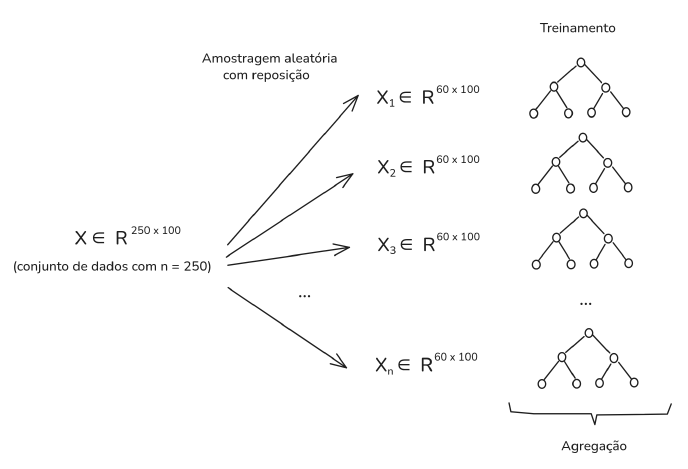
\includegraphics[scale=0.95]{pngs/RF_img.png}
\caption{Esquema simplificado do funcionamento de uma Floresta Aleatória.}
\label{fig:random_forest}
\end{center}
\end{figure}

\begin{figure}[htbp]
\begin{center}
	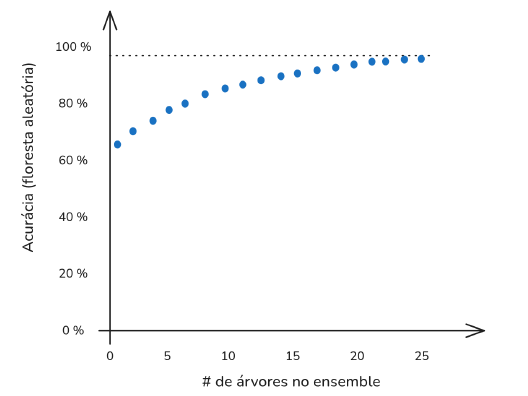
\includegraphics[scale=0.85]{pngs/manual_2.png}
\caption{Exemplo ilustrativo: 25 árvores com acurácia individual em torno de 65\% podem resultar em uma floresta com acurácia de aproximadamente 94\%.}
\label{fig:ensemble_acuracia}
\end{center}
\end{figure}

\subsection{XGBoost (eXtreme Gradient Boosting)}

O \textbf{boosting} é uma família de métodos em que os modelos são treinados \textbf{um após o outro}: cada novo modelo (por exemplo, uma árvore) é ajustado para corrigir os erros do modelo anterior, de modo que a combinação de todos forme um preditor forte a partir de vários preditores "fracos" \citep{geron2019maos, Levada2026}. O \textbf{gradient boosting} utiliza um modelo aditivo: na iteração \(m\),
\begin{equation}
F_m(\vec{x}) = F_{m-1}(\vec{x}) + \eta \, h_m(\vec{x}),
\end{equation}
onde \(h_m\) é um novo aprendiz fraco (por exemplo, uma árvore rasa) ajustado ao \textbf{gradiente negativo} da função de perda em relação à predição atual \(F_{m-1}\) --- ou seja, aos "resíduos" no espaço da perda \citep{geron2019maos}. A taxa de aprendizado \(\eta\) controla a contribuição de cada árvore (encolhimento, \textit{shrinkage}), reduzindo o risco de overfitting. O XGBoost (\textit{eXtreme Gradient Boosting}) aprimora esse esquema ao adicionar termos de regularização explícitos na função de custo (penalizando o número de folhas e os pesos das folhas) e ao utilizar uma expansão de Taylor de segunda ordem da perda para otimizar a atualização de cada árvore, o que resulta em implementação eficiente e alto desempenho \citep{geron2019maos}.

O XGBoost tornou-se muito popular em competições e aplicações práticas por sua precisão e velocidade. Em contraste com o Random Forest (que treina árvores em paralelo), o boosting é inerentemente sequencial, o que pode limitar o paralelismo em certas fases, mas o ganho de desempenho preditivo costuma compensar. \ia{Na \textit{pipeline} desta dissertação, o XGBoost é um dos quatro classificadores treinados e avaliados (Regressão Logística, Random Forest, XGBoost, CatBoost) (Capítulo 4).}

\subsection{CatBoost}

CatBoost (\textit{Categorical Boosting}) é um algoritmo de \textit{gradient boosting} baseado em árvores, desenvolvido pela Yandex, que incorpora inovações voltadas à robustez e à eficiência do treinamento.

Assim como o XGBoost, o CatBoost constrói árvores sequencialmente, minimizando uma função de perda por gradiente. Entretanto, difere em dois aspectos arquiteturais relevantes:

\begin{itemize}
	\item \textbf{\textit{Ordered Boosting}:} para calcular os resíduos de cada exemplo, o CatBoost utiliza apenas os modelos treinados com exemplos anteriores a ele (em uma permutação aleatória do conjunto), combatendo o \textit{target leakage} (vazamento de rótulo) --- situação em que a predição de um exemplo é influenciada pelo próprio rótulo durante o treinamento. Esse procedimento reduz o viés otimista na estimativa dos resíduos, especialmente em conjuntos pequenos ou moderados.

	\item \textbf{\textit{Oblivious Decision Trees}:} cada nível da árvore aplica a \textbf{mesma condição de divisão} a todos os nós daquele nível. Essa restrição produz árvores simétricas (ou "oblivious"), que são mais rápidas de avaliar e atuam como regularização estrutural, reduzindo o risco de \textit{overfitting}.
\end{itemize}

O CatBoost também possui tratamento nativo de variáveis categóricas --- codificando-as internamente sem necessidade de \textit{one-hot encoding} --- e opções para lidar com desbalanceamento de classes, como o parâmetro \textit{auto\_class\_weights='Balanced'}, que ajusta automaticamente os pesos das classes de forma inversamente proporcional à sua frequência.

A métrica de importância de variáveis padrão do CatBoost é o \textbf{\textit{PredictionValuesChange}}: para cada \textit{feature}, mede-se a mudança média nas predições do modelo ao longo de todos os \textit{splits} que a utilizam. Os valores são normalizados para que a soma seja igual a~100. \ia{Neste trabalho, CatBoost é utilizado junto com Regressão Logística, Random Forest e XGBoost para comparação de desempenho e robustez na classificação de curvas de luz (Capítulo~4).}

% -----------------------------------------------------------------------------
\section{Agrupamento não supervisionado: K-means}
\label{sec:kmeans}

O \textbf{K-means}, proposto originalmente por \citet{MacQueen1967}, é um algoritmo de \textbf{agrupamento} (clustering) não supervisionado: não usa rótulos; apenas particiona os dados em \(k\) grupos de modo a minimizar a soma dos quadrados das distâncias de cada ponto ao centróide do seu grupo \citep{geron2019maos, Levada2026}. A função objetivo, conhecida como \textit{Within-Cluster Sum of Squares} (WCSS) ou inércia, é
\begin{equation}
J = \sum_{i=1}^{k} \sum_{\vec{x} \in S_i} \|\vec{x} - \vec{\mu}_i\|^2,
\end{equation}
onde \(S_i\) é o conjunto de pontos atribuídos ao cluster \(i\) e \(\vec{\mu}_i\) é o centróide desse cluster. O algoritmo alterna dois passos: (1) \textbf{atribuição} --- cada ponto é atribuído ao centróide mais próximo; (2) \textbf{atualização} --- cada centróide é recalculado como a média aritmética dos pontos a ele atribuídos. O custo \(J\) não aumenta a cada iteração, de modo que o processo converge para um mínimo local \citep{geron2019maos, Levada2026}. Em aplicações em que \(k\) não é fixo, a inércia (WCSS) é frequentemente usada no \textbf{método do cotovelo} (gráfico de WCSS em função de \(k\)) para sugerir o número de clusters; índices como o de \textbf{Calinski-Harabasz} medem a razão entre dispersão inter e intra-cluster, indicando quão bem separados estão os grupos. Para mais detalhes sobre o funcionamento deste algoritmo, fica como recomendação o paper original: \citet{MacQueen1967}.

Nesta dissertação, o K-means \textbf{não} é usado como classificador de curvas, e sim como ferramenta para \textbf{extrair uma característica numérica}: aplica-se K-means com \(K=2\) aos valores do fluxo (ou do fluxo suavizado) de cada curva. Como não há rótulos, o algoritmo apenas descobre dois "níveis" típicos nos dados \citep{Levada2026}. Os dois centróides representam, grosso modo, o nível "fora da ocultação" e o nível "dentro da ocultação". A \textbf{distância entre os centróides} é então usada como mais uma entrada (feature) para o classificador: curvas com ocultação bem definida tendem a ter distância maior; curvas apenas ruidosas tendem a ter distância menor. O detalhe está no Capítulo 4. No uso aqui, \(k=2\) e a variável é unidimensional (fluxo), o que simplifica a interpretação.

% -----------------------------------------------------------------------------
\section{Algoritmos de otimização no treinamento}
\label{sec:otimizacao}

Em um projeto de ML supervisionado, a etapa de \textbf{treinamento} corresponde, como explicado anteriormente, a ajustar os parâmetros do modelo de modo a minimizar uma função de custo (ou perda) nos dados. Nas seções anteriores foram apresentados os modelos e suas funções de custo; aqui unificamos os \textbf{algoritmos} usados para obter o minimizador. A minimização pode ser feita por \textbf{solução analítica fechada}, quando existe fórmula explícita (como na regressão linear, Seção~\ref{sec:reglin_didatica}), ou por \textbf{algoritmos iterativos}, quando não há forma fechada. Os três esquemas mais recorrentes são resumidos a seguir; a Tabela~\ref{tab:otimizacao} indica em que contexto cada um aparece.

\textbf{1. Mínimos quadrados (solução fechada).} Conforme visto na regressão linear (Seção~\ref{sec:reglin_didatica}), modelos lineares com custo quadrático possuem minimizador analítico dado pela equação normal \(\vec{\theta}^* = (X^\top X)^{-1} X^\top \vec{y}\). Na Regressão Logística e em modelos não lineares, recorre-se a métodos iterativos.

\textbf{2. Gradiente descendente (método de primeira ordem).} O \textbf{gradiente} da função de custo indica a direção de maior crescimento do custo; para minimizar, atualiza-se os parâmetros na \textbf{direção oposta}, com passo controlado pela taxa de aprendizado \(\eta\):
\[
\vec{\theta}_{t+1} = \vec{\theta}_t - \eta \, \nabla_{\vec{\theta}} J(\vec{\theta}_t).
\]
As variantes principais distinguem-se pela quantidade de dados usada em cada atualização \citep{geron2019maos}: \textbf{Batch GD} utiliza todo o conjunto de treino (preciso, mas lento em grandes volumes); \textbf{Stochastic GD} (SGD) utiliza uma única instância aleatória por passo (rápido e capaz de escapar de mínimos locais, mas com trajetória errática); \textbf{Mini-batch GD} processa pequenos subconjuntos aleatórios, equilibrando estabilidade e eficiência. A convergência depende crucialmente de \(\eta\): se muito alta, o algoritmo pode divergir; se muito baixa, o treinamento torna-se excessivamente lento. Como vimos na Seção~\ref{sec:modelos_classificacao}, a Regressão Logística é ajustada por gradiente descendente; o mesmo esquema é usado em redes neurais e no gradient boosting (cada árvore é ajustada ao gradiente da perda).

\textbf{3. Métodos de segunda ordem (Newton e variantes).} O \textbf{método de Newton} utiliza o gradiente e a \textbf{Hessiana} da função de custo:
\[
\vec{\theta}_{t+1} = \vec{\theta}_t - H^{-1}(\vec{\theta}_t) \, \nabla_{\vec{\theta}} J(\vec{\theta}_t).
\]
Isso permite passos mais informados e convergência mais rápida perto do mínimo, às custas de calcular e inverter \(H\) a cada iteração (custo \(O(p^3)\) por passo). Variantes \textbf{quasi-Newton} (como BFGS) aproximam a Hessiana sem calculá-la explicitamente. O XGBoost utiliza uma \textbf{expansão de Taylor de segunda ordem} da perda para determinar a atualização ótima de cada árvore no gradient boosting \citep{geron2019maos}.

\begin{table}[htbp]
\centering
\small
\caption{Algoritmos de otimização e seu papel na etapa de treinamento em projetos de ML.}
\label{tab:otimizacao}
\begin{tabular}{@{}p{2.2cm}p{4.1cm}p{5.2cm}@{}}
\hline
\textbf{Família} & \textbf{Exemplo} & \textbf{Onde aparece} \\
\hline
Solução fechada & Mínimos quadrados (equação normal) & Regressão linear (Seção~\ref{sec:reglin_didatica}) \\
\hline
Primeira ordem (iterativo) & Gradiente descendente (Batch, SGD, Mini-batch) & Regressão Logística, redes neurais, gradient boosting \\
\hline
Segunda ordem (iterativo) & Newton, quasi-Newton (BFGS), Taylor & XGBoost (Taylor da perda); otimização convexa em geral \\
\hline
\end{tabular}
\end{table}

\ia{Com isso, o leitor dispõe de uma referência clara sobre o significado das "contas" envolvidas no treinamento de modelos de aprendizado de máquina. Inicialmente, apresentamos um modelo simples de Regressão Linear ajustado por meio do método dos mínimos quadrados e discutimos suas limitações. Em seguida, introduzimos a Regressão Logística (Seção~\ref{sec:modelos_classificacao}) como um exemplo direto de otimização por gradiente descendente. Por fim, abordamos os ensembles de árvores, que utilizam critérios de divisão para o aprendizado; no caso do XGBoost, o processo de otimização incorpora informações de segunda ordem da função de perda, resultando em atualizações mais eficientes} \citep{geron2019maos}.

% -----------------------------------------------------------------------------
\section{Engenharia de características e validação de modelos}
\label{sec:feature_validacao}

\subsection{Engenharia de características}

A criação e a seleção de \textbf{características numéricas} (atributos) a partir dos dados brutos são fundamentais para o sucesso do ML \citep{geron2019maos}, uma vez que essas variáveis representam a informação que será efetivamente utilizada pelos algoritmos para identificar padrões e realizar previsões.

Essa etapa inclui: (i)~escolher ou construir variáveis que capturem informação útil para a tarefa (por exemplo, estatísticas da curva de luz, derivadas, comparações entre segmentos); (ii)~combinar ou transformar variáveis existentes (médias móveis, suavização, testes estatísticos entre quartis, etc.). No Capítulo 4, descreve-se em detalhe o conjunto de features extraídas de cada curva de luz (amplitude, desvio padrão, max drawdown, distância entre centróides do K-means no fluxo, estatísticas de derivadas, \(p\)-valores entre quartis, entre outras). Essas grandezas formam o vetor \(\vec{x}\) de entrada dos classificadores.

\subsection{Métricas de avaliação para classificação binária}
\label{sec:metricas_avaliacao}

A avaliação de um classificador binário parte da \textbf{matriz de confusão}, que contabiliza os acertos e erros do modelo em relação aos rótulos verdadeiros. Sejam \(y_i \in \{0,1\}\) os rótulos reais e \(\hat{y}_i\) as predições; definem-se quatro contagens:

\begin{itemize}
	\item \textbf{Verdadeiro Positivo (TP):} $\hat{y}_i = 1$ e $y_i = 1$ (acerto na classe positiva).
	\item \textbf{Verdadeiro Negativo (TN):} $\hat{y}_i = 0$ e $y_i = 0$ (acerto na classe negativa).
	\item \textbf{Falso Positivo (FP):} $\hat{y}_i = 1$ e $y_i = 0$ (alarme falso).
	\item \textbf{Falso Negativo (FN):} $\hat{y}_i = 0$ e $y_i = 1$ (evento perdido).
\end{itemize}

A partir dessas contagens, as métricas mais utilizadas em classificação binária são:

\textbf{Acurácia} --- fração de predições corretas sobre o total:

\begin{equation}
\text{Acurácia} = \frac{TP + TN}{TP + TN + FP + FN}.
\end{equation}

A acurácia é intuitiva, mas pode ser enganosa em conjuntos desbalanceados. 

\textbf{Exemplo numérico:} considere 100 curvas de luz, das quais 10 contêm ocultação (positivas) e 90 não (negativas). Um classificador que \textbf{sempre} prediz "negativo" acerta 90 das 100 curvas --- acurácia de 90\% --- mas não detecta \textit{nenhuma} ocultação ($\text{sensibilidade} = 0$). Esse paradoxo evidencia que, em cenários desbalanceados, a acurácia sozinha é insuficiente para avaliar o modelo.

\textbf{Precisão} (\textit{Precision}) --- entre os exemplos classificados como positivos, qual fração é realmente positiva:
\begin{equation}
\text{Precisão} = \frac{TP}{TP + FP}.
\end{equation}

\textbf{Sensibilidade} (\textit{Recall}, ou sensibilidade) --- entre os exemplos verdadeiramente positivos, qual fração foi corretamente detectada:
\begin{equation}
\text{Sensibilidade} = \frac{TP}{TP + FN}.
\end{equation}

\textbf{F1-score} --- média harmônica de precisão e sensibilidade, oferecendo um compromisso entre ambas:
\begin{equation}
F_1 = 2 \cdot \frac{\text{Precisão} \cdot \text{Sensibilidade}}{\text{Precisão} + \text{Sensibilidade}} = \frac{2\,TP}{2\,TP + FP + FN}.
\end{equation}

\textbf{F$_\beta$-score} --- generalização do F1-score que permite atribuir peso diferente à sensibilidade:
\begin{equation}
F_\beta = (1 + \beta^2) \cdot \frac{\text{Precisão} \cdot \text{Sensibilidade}}{\beta^2 \cdot \text{Precisão} + \text{Sensibilidade}}.
\end{equation}
Para $\beta > 1$, o $F_\beta$ penaliza mais os falsos negativos (favorecendo a sensibilidade); para $\beta < 1$, penaliza mais os falsos positivos. Em aplicações de triagem científica, como a detecção de ocultações estelares, $\beta = 2$ é uma escolha natural, pois o custo de perder um evento genuíno (FN) é maior que o de investigar um alarme falso (FP) \citep{Saito2015}.

\textbf{AUC-ROC} (\textit{Area Under the Receiver Operating Characteristic Curve}) --- mede a capacidade discriminativa do modelo ao longo de todos os limiares de decisão possíveis. A curva ROC plota a \textbf{taxa de verdadeiros positivos} (sensibilidade) contra a \textbf{taxa de falsos positivos} ($FP/(FP+TN)$) para cada limiar $\tau$. A área sob essa curva (AUC) varia de 0,5 (classificador aleatório) a 1,0 (classificador perfeito), como mostrado na imagem \ref{fig:roc_auc}. A AUC-ROC é útil por ser invariante ao limiar escolhido, mas pode ser otimista em conjuntos desbalanceados \citep{Saito2015}.

\begin{figure}[h!]
\begin{center}
	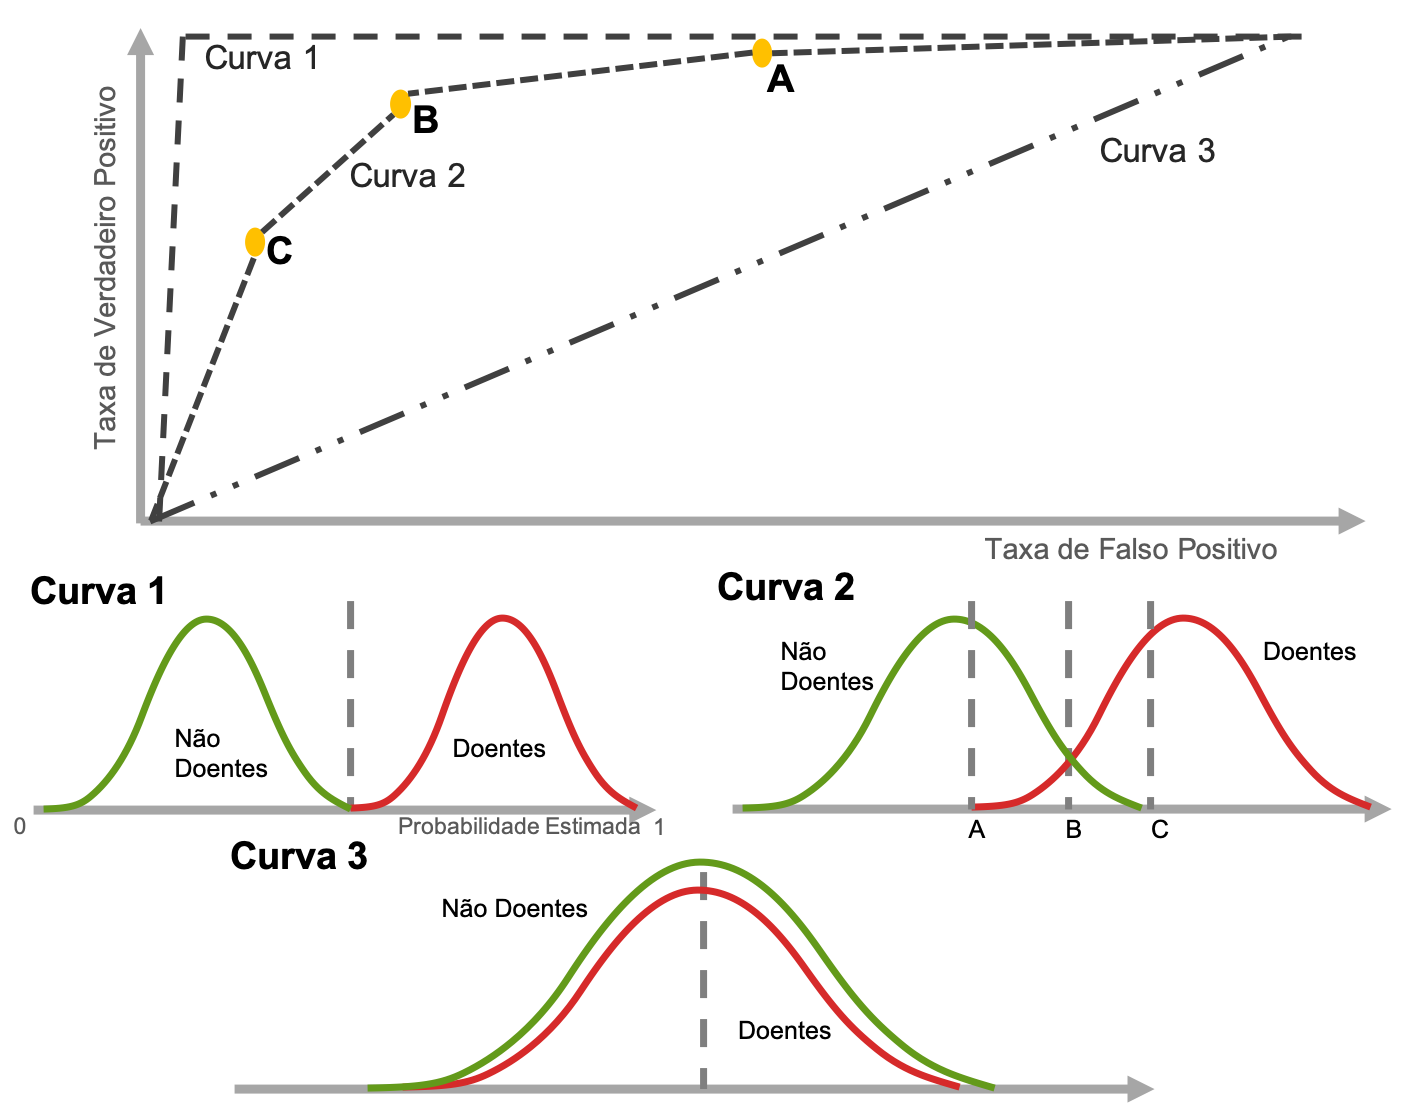
\includegraphics[width=0.75\textwidth]{pngs/roc_curvas_todas_ref_httpscienciaenegocios.comcurva-roc-e-auc-em-machine-learning.png}
\caption{Exemplos de curvas ROC para classificadores de diferentes qualidades: quanto mais a curva se aproxima do canto superior esquerdo (maior área sob a curva, AUC), melhor a capacidade discriminativa do modelo; a diagonal corresponde a um classificador aleatório (AUC = 0,5). Um exemplo intuitivo é um teste médico que classifica pacientes como doentes ou saudáveis: a taxa de verdadeiros positivos mede a fração de doentes corretamente identificados, enquanto a taxa de falsos positivos mede a fração de saudáveis erroneamente apontados como doentes. Variar o limiar de decisão move o teste ao longo da curva, negociando a detecção de mais doentes contra um número maior de alarmes falsos. Fonte: adaptado de \emph{Ciência e Negócios}\protect\footnotemark.}
\label{fig:roc_auc}
\end{center}
\end{figure}
\footnotetext{Disponível em: \url{https://cienciaenegocios.com/curva-roc-e-auc-em-machine-learning}. Acesso em: 6 abr. 2026.}

\textbf{Curva Precisão-Sensibilidade} (\textit{Precision-Recall}) --- alternativa à curva ROC, recomendada quando a classe positiva é rara ou quando o custo dos erros é assimétrico \citep{Saito2015}. Plota a precisão contra a sensibilidade para cada limiar~$\tau$. A área sob a curva PR (AUC-PR) é mais informativa que a AUC-ROC em cenários desbalanceados, pois não é inflada por verdadeiros negativos abundantes.

Nesta dissertação, os modelos são avaliados por acurácia, precisão, sensibilidade, F1-score e AUC-ROC no conjunto de teste (Capítulo~5). Para a análise de ajuste de limiar, utilizam-se também o $F_2$-score e a curva precision-recall.

\subsection{Overfitting, underfitting e o compromisso entre viés e variância}
\label{sec:overfitting}

A identificação de \textbf{sobreajuste} (overfitting) e \textbf{subajuste} (underfitting) baseia-se na comparação do desempenho do modelo nos dados usados no treinamento versus nos dados reservados para teste ou validação \citep{geron2019maos}. Em termos intuitivos: \textbf{sobreajuste} ocorre quando o modelo "decora" os dados de treino (incluindo o ruído) e deixa de generalizar --- o erro no treino fica muito baixo, mas o erro em dados novos permanece alto. \textbf{Subajuste} ocorre quando o modelo é simples demais e não captura o padrão verdadeiro dos dados --- tanto o erro de treino quanto o de validação ficam altos. 

O erro de generalização pode ser decomposto em \textbf{viés}, \textbf{variância} e \textbf{ruído irredutível} \citep{Deisenroth2019, Levada2026}. Formalmente, para um modelo $\hat{f}$ treinado em diferentes amostras do mesmo processo gerador, o erro quadrático médio esperado em um ponto $\vec{x}$ é:
\begin{equation}
\mathbb{E}\!\left[(y - \hat{f}(\vec{x}))^2\right] = \text{Viés}^2[\hat{f}(\vec{x})] + \text{Var}[\hat{f}(\vec{x})] + \sigma^2,
\label{eq:bias_variance}
\end{equation}
onde $\text{Viés}^2[\hat{f}] = \left(\mathbb{E}[\hat{f}(\vec{x})] - f(\vec{x})\right)^2$ mede o erro sistemático do modelo (quão longe a predição média está do valor verdadeiro), $\text{Var}[\hat{f}]$ mede a sensibilidade do modelo a flutuações nos dados de treino, e $\sigma^2$ é a variância do ruído intrínseco aos dados (irredutível por qualquer modelo). Modelos muito simples tendem a alto viés (subajuste); modelos muito flexíveis tendem a alta variância (sobreajuste). O objetivo prático é encontrar um equilíbrio que minimize o erro total.

\textbf{Diagnóstico.} O sinal mais claro de sobreajuste é um erro muito baixo no treino e um erro alto no teste ou validação (não generalizou). Esse diagnóstico é feito graficamente pelas \textbf{curvas de aprendizado} (Seção~\ref{sec:curvas_aprendizado}): o sobreajuste aparece como um \textbf{gap} entre a curva de treino e a de validação, enquanto o subajuste mantém ambas próximas e em um \textbf{platô alto} de erro.

A \textbf{validação cruzada} --- detalhada na Seção~\ref{sec:validacao_modelos} --- complementa esse diagnóstico ao fornecer uma estimativa robusta do erro de generalização (média e desvio padrão sobre várias divisões dos dados), facilitando perceber quando o modelo começou a sobreajustar \citep{geron2019maos}.

\ia{Em resumo: \textbf{sobreajuste} (overfitting) significa que o modelo se ajustou demais aos dados de treino (incluindo o ruído) e perde capacidade de generalizar; soluções típicas são obter mais dados, simplificar o modelo ou usar regularização (penalizar parâmetros grandes). \textbf{Subajuste} (underfitting) significa que o modelo é simples demais e não captura o padrão dos dados; as soluções envolvem aumentar a complexidade do modelo ou enriquecer as características de entrada. Os \textbf{hiperparâmetros} (por exemplo, força da regularização, profundidade máxima das árvores) controlam esse equilíbrio e podem ser escolhidos via validação cruzada.}

A \textbf{regularização} restringe a liberdade do modelo (por exemplo, penalidade \(\ell_2\) na Regressão Logística ou limites de profundidade e número de folhas nas árvores), sendo controlada por hiperparâmetros que podem ser ajustados via validação cruzada \citep{geron2019maos}. Outras formas incluem a \textbf{parada antecipada}: interromper o treinamento quando o erro no conjunto de validação deixa de melhorar, evitando que o modelo "decore" o ruído do treino. Nesta dissertação, o foco está na penalização de pesos em modelos lineares (Ridge/Lasso) e nos critérios de parada e poda nas árvores. A regularização \(\ell_1\) e \(\ell_2\) é \textbf{sensível à escala} das variáveis de entrada: atributos em escalas maiores tendem a receber pesos menores pela penalização. Em geral, recomenda-se \textbf{padronizar} as variáveis (subtrair a média e dividir pelo desvio padrão) antes de aplicar Ridge ou Lasso. 

Na \textit{pipeline} desta dissertação, as features não são padronizadas antes de todos os treinos (Capítulo 4); a justificativa é discutida naquele capítulo.

\subsection{Curvas de aprendizado}
\label{sec:curvas_aprendizado}

As \textbf{curvas de aprendizado} mostram o desempenho do modelo (acurácia ou erro) em função do tamanho do conjunto de treino (ou do número de épocas); são a ferramenta gráfica que torna visível o equilíbrio viés--variância discutido acima e auxiliam na decisão de coletar mais dados ou alterar a complexidade do modelo.

A Figura~\ref{fig:learning_curves} ilustra o conceito com curvas de aprendizado reais de três classificadores (XGBoost, Random Forest e Árvore de Decisão) em uma tarefa de classificação. Em cada painel, a curva superior é o desempenho no \textbf{treino} e a inferior o desempenho em \textbf{validação cruzada}, ambos em função do número de amostras de treino. Dois padrões didáticos aparecem: (i)~a curva de validação \textbf{sobe} à medida que mais dados ficam disponíveis e tende a um \textbf{platô}, ponto a partir do qual coletar mais exemplos pouco acrescenta; (ii)~o \textbf{intervalo} (\textit{gap}) entre a curva de treino (quase perfeita) e a de validação mede o \textbf{sobreajuste} --- quanto maior o vão, mais o modelo decorou o treino em vez de generalizar. Um modelo bem ajustado é aquele cujas duas curvas convergem para um patamar alto com vão pequeno.

\begin{figure}[h!]
\begin{center}
	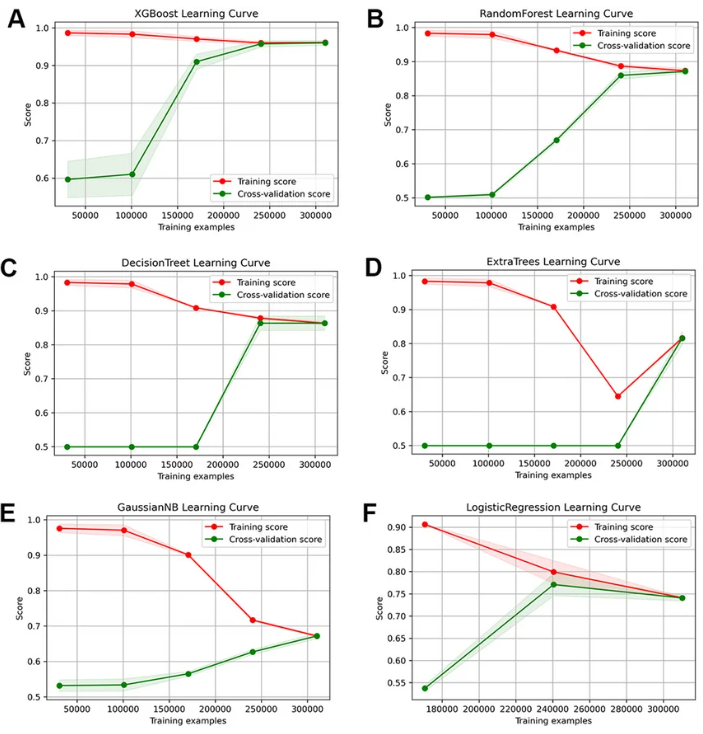
\includegraphics[width=0.8\textwidth]{pngs/Learning-curves-of-models-with-training-data-A-XGBoost-B-Random-Forest-C.png}
\caption{Exemplo de curvas de aprendizado (dados genéricos, não referentes a curvas de luz de ocultação) para três classificadores: (A)~XGBoost, (B)~Random Forest e (C)~Árvore de Decisão. Em cada painel, compara-se o desempenho no conjunto de treino com o obtido em validação cruzada, em função do número de amostras de treino; o vão entre as duas curvas indica o grau de sobreajuste, e o platô da curva de validação indica a partir de quando mais dados deixam de melhorar o modelo. Fonte: adaptado de \emph{ResearchGate}\protect\footnotemark.}
\label{fig:learning_curves}
\end{center}
\end{figure}
\footnotetext{Disponível em: \url{https://www.researchgate.net/figure/Learning-curves-of-models-with-training-data-A-XGBoost-B-Random-Forest-C_fig2_374986649}. Acesso em: 6 abr. 2026.}

\subsection{Validação de modelos}
\label{sec:validacao_modelos}

Para estimar o desempenho em dados não vistos e evitar otimismo, é essencial separar os dados usados no treino daqueles usados na avaliação \citep{geron2019maos}. Imagine que treinamos o modelo usando todas as curvas de luz disponíveis e depois o avaliamos nessas mesmas curvas. O resultado seria enganosamente bom. Para estimar honestamente o desempenho, é preciso reservar dados que o modelo nunca viu. A \textbf{validação cruzada} sistematiza esse processo: em vez de uma única divisão treino/teste (que pode ser sortuda ou azarada), roda-se o experimento $k$ vezes, cada vez deixando uma fatia diferente de fora. A média dos $k$ resultados é uma estimativa muito mais robusta do erro de generalização.

\begin{figure}[htbp]
\begin{center}
	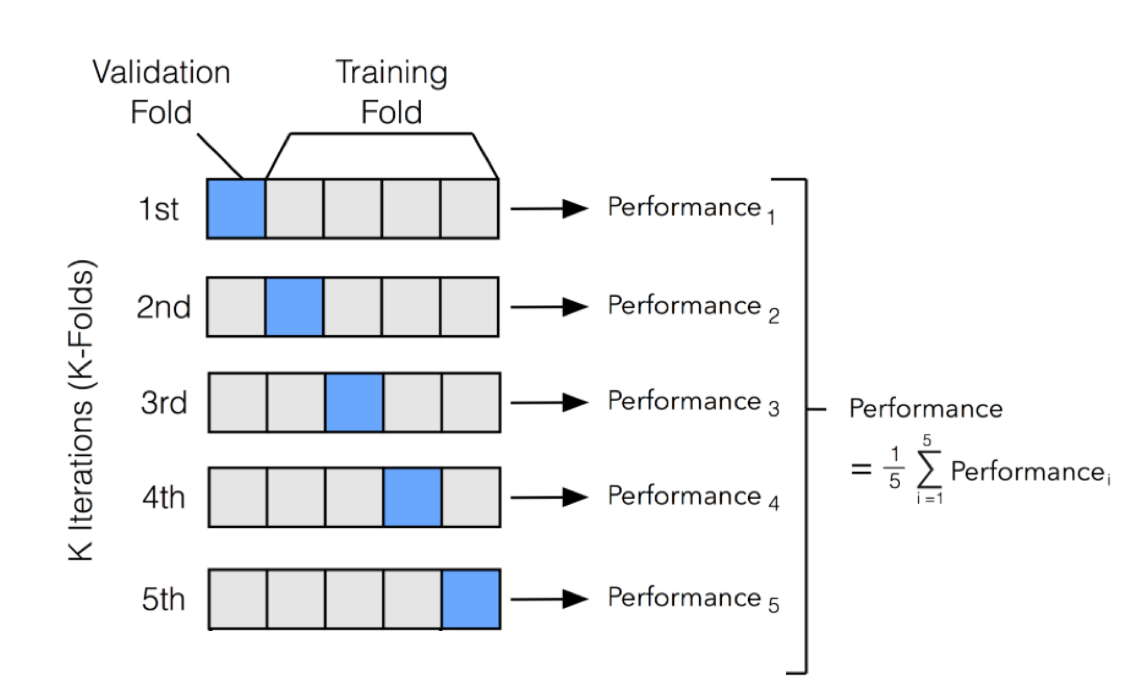
\includegraphics[width=0.75\textwidth]{pngs/kfold.png}
\caption{Esquema da validação cruzada com $k=5$: em cada rodada, uma fatia diferente (em destaque) é usada como conjunto de validação, e as demais como treino. Fonte: adaptado de Nishad~(2023)\protect\footnotemark.}
\label{fig:kfold}
\end{center}
\end{figure}
\footnotetext{Disponível em: 

\url{https://medium.com/@nishad009adi/k-fold-cross-validation-with-simple-example-e023bb2e2d43}. Acesso em: 6 abr. 2026.}

As estratégias mais comuns são:

\begin{itemize}
	\item \textbf{Conjunto de teste:} uma fração dos dados é reservada e nunca usada no treino; o desempenho nesse conjunto fornece uma estimativa do erro de generalização.
	\item \textbf{Validação cruzada (k-fold):} os dados são divididos em \(k\) partes (dobras); em cada rodada, \(k-1\) dobras são usadas para treino e uma para validação; a métrica final é a média sobre as \(k\) rodadas. Isso dá uma estimativa mais estável do desempenho e é útil para comparar modelos ou escolher hiperparâmetros (parâmetros do algoritmo que não são ajustados pelo treinamento, como a força da regularização).
	\item \textbf{Validação cruzada estratificada:} quando as classes são desbalanceadas (por exemplo, poucas curvas com ocultação e muitas sem), a divisão aleatória simples pode produzir dobras em que uma das classes está sub ou sobrerrepresentada. A validação \textbf{estratificada} preserva a proporção de cada classe em cada dobra, tornando a estimativa mais confiável \citep{geron2019maos}. Na detecção de ocultações, o uso de divisão estratificada é recomendado.
	\item \textbf{Busca em grade:} para escolher hiperparâmetros, avalia-se um conjunto de combinações (a "grade") e escolhe-se a que maximiza a métrica de validação.
\end{itemize}

Na \textit{pipeline} desta dissertação (Capítulo 4), a divisão treino/teste é feita de forma estratificada (mantendo a proporção de positivas e negativas em cada parte) ou por seleção manual de curvas para o teste. As métricas (acurácia, precisão, sensibilidade, F1-score, AUC-ROC) são calculadas no \textbf{conjunto de teste} --- dados que o modelo nunca viu durante o treinamento. \ia{Com isso, o capítulo fornece a base conceitual necessária para interpretar a metodologia e os resultados descritos no Capítulo 4.}
